% Provenance (never printed): see sources/outline_sources.md (Year 2: Goldschmidt's
% classification; the chondritic Earth; core, mantle and crust compositions; trace
% elements and normalised diagrams). Curves from figdata/bachelor-2/geochem.py; exercise
% and problem values in the Book 4 scratch calculator calc/ch03.py.
\chapter{Unsur-Unsur di dalam Bumi}\label{ch:b2:elements-in-the-earth}

Satu ton batuan benua mengandung sekitar satu setengah miligram
emas. Satu ton \omterm{def:b2:planet-formation-meteorites:chondrule}{kondrit berkarbon} dari bab sebelumnya, batu paling
primitif yang jatuh dari langit, mengandung sekitar seratus kali lebih banyak. Bumi
dihimpun dari bahan semacam itu, sehingga emas tidak hilang dari
Bumi: emas itu berada di tempat lain. Gabungkan taksiran komposisi inti dan
Bumi silikat dengan massa inti, maka lebih dari 99 persen emas
Bumi ternyata berada di inti, tempat emas itu tenggelam bersama besi pada awal
sejarah Bumi. Emas termasuk satu keluarga unsur yang mengikuti besi
logam; unsur lain mengikuti sulfida, yang lain lagi batuan silikat, dan yang lainnya lolos
ke udara. Bab ini memilah unsur-unsur ke dalam keluarga-keluarga ini, memakai
\omterm{def:b2:planet-formation-meteorites:chondrule}{kondrit} untuk merekonstruksi komposisi Bumi secara keseluruhan dan menimbang
intinya, menguraikan komposisi mantel, kerak samudra, dan
kerak benua, serta memperkenalkan \omterm{def:b2:elements-in-the-earth:trace}{unsur jejak} dan diagram-diagram yang dipakai
ahli geokimia untuk membaca sejarah sebuah batuan.
% ledger: rg03:ucc-trace, lodders:ci-table, mcd03:core, ms95:pm-trace, data:prem

\begin{recall}
Bumi memiliki inti logam, sebagian besar besi, di bawah mantel silikat dan kerak
yang tipis; seismologi memberikan jari-jari dan massa jenis setiap lapisan, dan inti itu
5 hingga 10 persen kurang rapat daripada besi murni pada tekanan dan suhu yang sama,
sehingga diperlukan unsur ringan di dalamnya: silikon, belerang, karbon,
oksigen, dan hidrogen adalah calonnya (volume Tahun 1). Keelektronegatifan
sebuah unsur mengukur seberapa kuat atom-atomnya menarik
elektron sebuah ikatan, dan jari-jari sebuah ion bergantung pada muatannya dan pada
jumlah tetangganya (volume Tahun 1 buku kimia). Koefisien
partisi adalah perbandingan konsentrasi suatu zat dalam dua fase yang berada dalam
kesetimbangan (volume Tahun 1 buku kimia). \omterm{def:b2:planet-formation-meteorites:chondrule}{Kondrit}, \omterm{def:b2:planet-formation-meteorites:chondrule}{kondrit
berkarbon}, dan \omterm{def:b2:planet-formation-meteorites:condensation}{urutan kondensasi} telah diperkenalkan pada
\cref{ch:b2:planet-formation-meteorites}.
\end{recall}
% ledger: badro:core

\section{Klasifikasi Goldschmidt}

Ketika benda kondritik melebur, materinya terpisah menjadi cairan-cairan yang tidak saling
bercampur: logam besi dan nikel yang rapat, cairan sulfida jika belerangnya cukup, dan
lelehan silikat, dengan fase gas di atasnya. Setiap unsur mendistribusikan dirinya di antara
fase-fase ini menurut sifat kimianya, dan partisi yang sama terlihat dalam
peleburan bijih, ketika besi cair, matte sulfida, dan terak silikat terpisah di dalam
tanur.

\begin{definition}[Klasifikasi Goldschmidt]
\label{def:b2:elements-in-the-earth:goldschmidt}
Yang disebut \emph{klasifikasi Goldschmidt}\index{klasifikasi Goldschmidt} memilah
unsur-unsur menurut fase yang disukainya dalam benda yang terpisah menjadi logam,
sulfida, silikat, dan gas. Yang disebut \emph{unsur litofil}\index{unsur litofil}
menyukai silikat dan oksida; \emph{unsur siderofil}\index{unsur siderofil}
menyukai besi logam; \emph{unsur
kalkofil}\index{unsur kalkofil} menyukai sulfida; \emph{unsur
atmofil}\index{unsur atmofil} tetap berada dalam gas, sebagai gas atau senyawa
volatil.
\end{definition}

Kelas-kelas itu mengikuti kimia ikatan. \omterm{def:b2:elements-in-the-earth:goldschmidt}{Unsur litofil}, seperti logam
alkali dan alkali tanah, aluminium, titanium, atau tanah jarang, mudah
melepaskan elektronnya kepada oksigen, yang jauh lebih elektronegatif, dan
membentuk ikatan ionik dengannya. \omterm{def:b2:elements-in-the-earth:goldschmidt}{Unsur siderofil}, yaitu logam golongan platina, emas,
nikel, dan kobalt, memiliki keelektronegatifan yang dekat dengan besi, berikatan lemah
dengan oksigen, dan larut dalam logam. \omterm{def:b2:elements-in-the-earth:goldschmidt}{Unsur kalkofil}, di antaranya tembaga, seng, timbal,
perak, dan kadmium, membentuk ikatan dengan belerang yang lebih kovalen.
\omterm{def:b2:elements-in-the-earth:goldschmidt}{Unsur atmofil} adalah gas mulia, nitrogen, dan hidrogen. Banyak
unsur termasuk dua kelas, bergantung pada kondisinya: besi sendiri
siderofil dalam benda yang kaya logam dan litofil dalam mantel yang teroksidasi, tempat besi
berada dalam olivin dan piroksen; wolfram dan molibdenum siderofil di
Bumi, tetapi sebagian besar keduanya tetap berada di mantel (gambar di bawah).

\begin{omfigure}
\centering
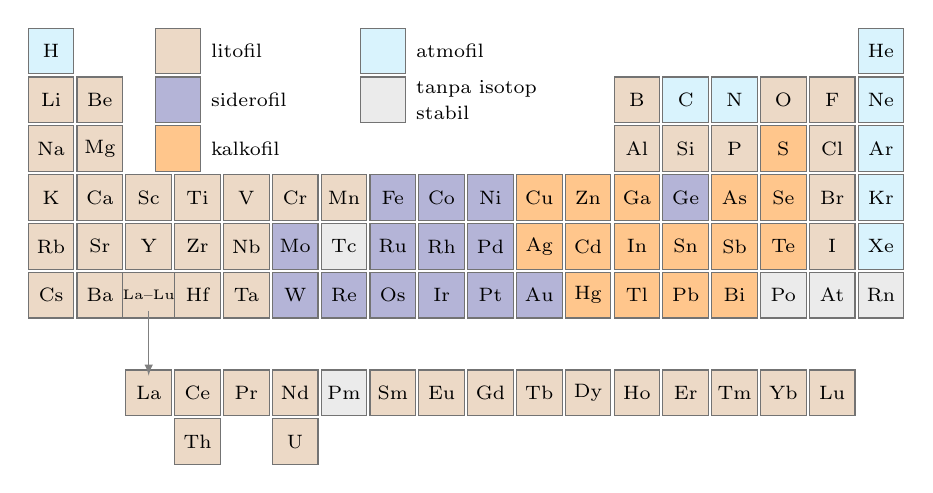
\begin{tikzpicture}[x=0.62cm, y=-0.62cm,
  lith/.style={fill=brown!30}, sid/.style={fill=blue!30!gray!45},
  chal/.style={fill=orange!45}, atm/.style={fill=cyan!15}, none/.style={fill=black!8},
  cell/.style={draw=black!55, minimum size=0.58cm, inner sep=0pt, font=\scriptsize}]
\foreach \s/\c/\r/\k in {H/1/1/atm, He/18/1/atm,
  Li/1/2/lith, Be/2/2/lith, B/13/2/lith, C/14/2/atm, N/15/2/atm, O/16/2/lith,
  F/17/2/lith, Ne/18/2/atm,
  Na/1/3/lith, Mg/2/3/lith, Al/13/3/lith, Si/14/3/lith, P/15/3/lith, S/16/3/chal,
  Cl/17/3/lith, Ar/18/3/atm,
  K/1/4/lith, Ca/2/4/lith, Sc/3/4/lith, Ti/4/4/lith, V/5/4/lith, Cr/6/4/lith,
  Mn/7/4/lith, Fe/8/4/sid, Co/9/4/sid, Ni/10/4/sid, Cu/11/4/chal, Zn/12/4/chal,
  Ga/13/4/chal, Ge/14/4/sid, As/15/4/chal, Se/16/4/chal, Br/17/4/lith, Kr/18/4/atm,
  Rb/1/5/lith, Sr/2/5/lith, Y/3/5/lith, Zr/4/5/lith, Nb/5/5/lith, Mo/6/5/sid,
  Tc/7/5/none, Ru/8/5/sid, Rh/9/5/sid, Pd/10/5/sid, Ag/11/5/chal, Cd/12/5/chal,
  In/13/5/chal, Sn/14/5/chal, Sb/15/5/chal, Te/16/5/chal, I/17/5/lith, Xe/18/5/atm,
  Cs/1/6/lith, Ba/2/6/lith, Hf/4/6/lith, Ta/5/6/lith, W/6/6/sid, Re/7/6/sid,
  Os/8/6/sid, Ir/9/6/sid, Pt/10/6/sid, Au/11/6/sid, Hg/12/6/chal, Tl/13/6/chal,
  Pb/14/6/chal, Bi/15/6/chal, Po/16/6/none, At/17/6/none, Rn/18/6/none,
  La/3/8/lith, Ce/4/8/lith, Pr/5/8/lith, Nd/6/8/lith, Pm/7/8/none, Sm/8/8/lith,
  Eu/9/8/lith, Gd/10/8/lith, Tb/11/8/lith, Dy/12/8/lith, Ho/13/8/lith,
  Er/14/8/lith, Tm/15/8/lith, Yb/16/8/lith, Lu/17/8/lith,
  Th/4/9/lith, U/6/9/lith}
  \node[cell, \k] at (\c,\r) {\s};
\node[cell, lith, minimum width=0.58cm] at (3,6) {\tiny La--Lu};
\draw[black!50, -latex] (3,6.32) -- (3,7.65);
% legend
\foreach \k/\t/\x/\y in {lith/litofil/3.6/1, sid/siderofil/3.6/2,
  chal/kalkofil/3.6/3, atm/atmofil/7.8/1, none/{\shortstack[l]{tanpa isotop\\stabil}}/7.8/2}
  \node[cell, \k, label={[font=\scriptsize]0:\t}] at (\x,\y) {};
\end{tikzpicture}
\par\smallskip{\small Kelas-kelas Goldschmidt unsur-unsur stabil serta torium dan uranium, yang isotop berumur panjangnya bertahan sejak kelahiran Bumi, diwarnai menurut kelas
yang dominan di Bumi; unsur-unsur baris tanah jarang berada dalam kotak
La--Lu. Beberapa unsur termasuk dua kelas: besi, nikel, dan kobalt juga
litofil dalam mantel yang teroksidasi; karbon juga siderofil, fosfor
siderofil dalam \omterm{def:b2:planet-formation-meteorites:fall-find}{meteorit}.}
\end{omfigure}

\section{Bumi kondritik}

Tak seorang pun dapat mengambil sampel Bumi secara keseluruhan: inti tidak terjangkau, dan
mantel hanya mencapai permukaan dalam bentuk pecahan. Komposisi Bumi total
karena itu dibangun dari dua bukti: \omterm{def:b2:planet-formation-meteorites:fall-find}{meteorit}, yang menjadi sampel
bahan pembentuk planet-planet, serta batuan mantel dan
lelehan yang berasal darinya.

\begin{definition}[Kondrit CI]\label{def:b2:elements-in-the-earth:ci}
Yang disebut \emph{kondrit CI}\index{kondrit CI} adalah anggota kelompok
\omterm{def:b2:planet-formation-meteorites:chondrule}{kondrit berkarbon} yang dinamai menurut \omterm{def:b2:planet-formation-meteorites:fall-find}{meteorit} Ivuna: batu hitam yang rapuh,
yang hampir seluruhnya tersusun atas matriks berbutir halus, kaya mineral yang mengandung air dan
karbon, nyaris tanpa \omterm{def:b2:planet-formation-meteorites:chondrule}{kondrul}. Selain hidrogen, karbon, nitrogen, oksigen, dan
gas mulia, komposisinya adalah yang paling dekat dengan fotosfer Matahari di antara semua bahan
yang dikenal; \omterm{def:b2:planet-formation-meteorites:chondrule}{kondrit} CI adalah komposisi acuan geokimia.
\end{definition}

Kelompok ini terdiri atas lima \omterm{def:b2:planet-formation-meteorites:fall-find}{meteorit}, semuanya \omterm{def:b2:planet-formation-meteorites:fall-find}{meteorit jatuhan}: Alais (1806), Orgueil
(1864), Tonk (1911), Ivuna (1938), dan Revelstoke (1965); Orgueil yang terbesar,
empat belas kilogram. Komposisi yang ditetapkan untuk kelompok ini adalah rata-rata berbobot
dari analisis-analisisnya, unsur demi unsur; nilai-nilai yang dipakai dalam bab ini
dikutip di tempat diperlukan.
% ledger: lodders:ci-table

\begin{definition}[Unsur refraktori dan unsur volatil]
\label{def:b2:elements-in-the-earth:volatility}
Yang disebut \emph{unsur refraktori}\index{unsur refraktori} adalah unsur yang \omterm{def:b2:planet-formation-meteorites:condensation}{suhu kondensasi}
50 persennya (\cref{ch:b2:planet-formation-meteorites}) terletak di atas
\omterm{def:b2:planet-formation-meteorites:condensation}{suhu kondensasi} magnesium, silikon, dan besi, \qtyrange{1310}{1340}{K} pada
\qty{e-4}{bar}; yang disebut
\emph{unsur volatil}\index{unsur volatil} adalah unsur yang \omterm{def:b2:planet-formation-meteorites:condensation}{suhu kondensasinya}
terletak di bawahnya.
\end{definition}

Kandungan magnesium dipakai sebagai tolok ukur. Magnesium bersifat litofil, mengembun
bersama sebagian besar batuan, dan tidak masuk ke inti, sehingga perbandingan suatu unsur
terhadap magnesium dalam Bumi silikat, dibagi perbandingan yang sama dalam \omterm{def:b2:elements-in-the-earth:ci}{kondrit CI},
mengukur seberapa banyak unsur itu dipertahankan Bumi silikat relatif terhadap
bahan awal yang kondritik. Air, karbon, dan senyawa volatil lain yang
dikandung \omterm{def:b2:elements-in-the-earth:ci}{kondrit CI}, yang tidak dipertahankan Bumi, saling meniadakan dalam perbandingan itu.

\begin{definition}[Bumi silikat total, mantel primitif]
\label{def:b2:elements-in-the-earth:bse}
Yang disebut \emph{Bumi silikat total}\index{Bumi silikat total} adalah Bumi tanpa
intinya: mantel, kerak, samudra, dan atmosfer bersama-sama, seolah-olah semuanya
tercampur. Komposisi yang sama disebut \emph{mantel primitif}\index{mantel primitif}:
mantel sebagaimana keadaannya setelah inti terbentuk dan sebelum kerak apa pun
diekstraksi darinya.
\end{definition}

Taksiran \omterm{def:b2:elements-in-the-earth:bse}{mantel primitif} bertumpu pada batuan mantel yang paling sedikit kehilangan
lelehan, yaitu peridotit yang terbawa ke atas sebagai xenolit dalam lava (foto di bawah) atau
tersingkap di sabuk pegunungan, dan pada anggapan bahwa \omterm{def:b2:elements-in-the-earth:goldschmidt}{unsur litofil} refraktori
berada dalam proporsi kondritik satu sama lain. Salah satu hasil yang banyak dipakai, dengan
magnesium 22.8, silikon 21.0, dan besi 6.26 persen massa, diberikan dalam
tabel komposisi lebih lanjut.
% ledger: ms95:pm-trace, ms95:pm-oxides

\begin{omfigure}
\centering
\begin{minipage}{0.48\linewidth}
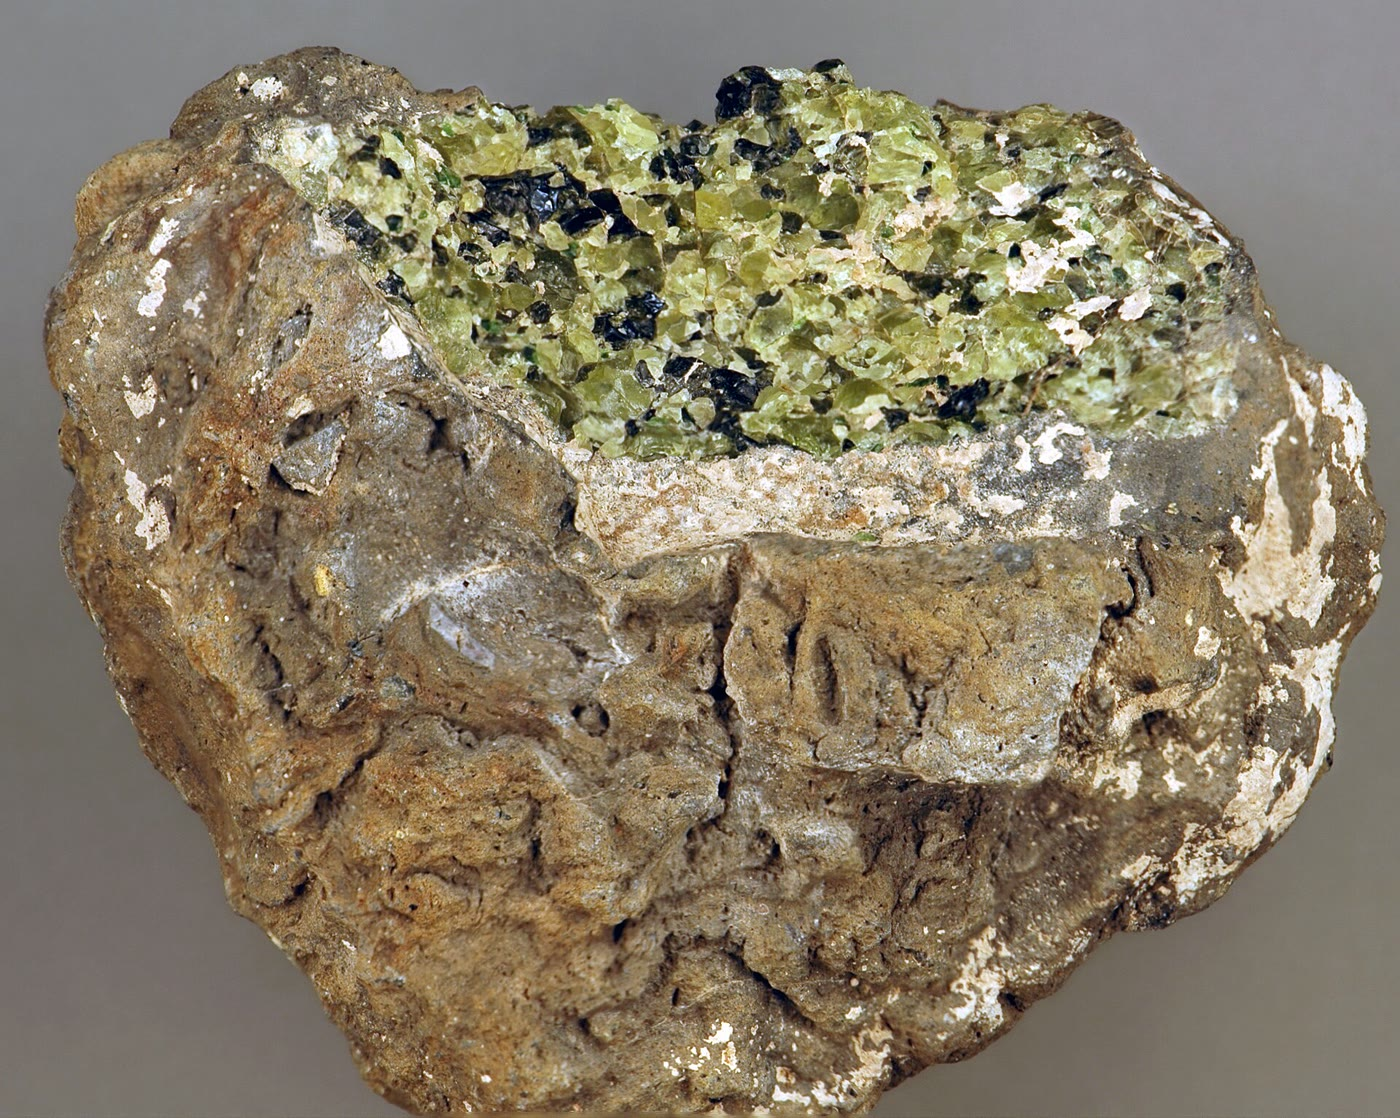
\includegraphics[width=\linewidth]{images/book4/b2-lherzolite-xenolith.jpg}
\end{minipage}\hfill
\begin{minipage}{0.48\linewidth}
{\small Sebuah nodul peridotit mantel (lherzolit) dalam lava basal dari
Kilbourne Hole, New Mexico, berdiameter \qty{7.4}{cm} pada bagian terlebarnya: olivin
kuning kehijauan dengan piroksen gelap. Lava itu merenggutnya dari mantel atas dan membawanya
ke permukaan. James St.~John, CC BY 2.0.}
\end{minipage}
\end{omfigure}

Gambar di bawah membandingkan Bumi silikat ini dengan \omterm{def:b2:elements-in-the-earth:ci}{kondrit CI}, unsur demi
unsur, terhadap \omterm{def:b2:planet-formation-meteorites:condensation}{suhu kondensasi} dari bab sebelumnya. Gambar itu memilah
unsur-unsur dengan cara yang tidak dapat dilakukan bukti lain. \omterm{def:b2:elements-in-the-earth:goldschmidt}{Unsur litofil}
refraktori, dari zirkonium dan tanah jarang hingga stronsium dan barium, semuanya
berada pada tingkat yang sama, dalam selisih dua puluh persen satu sama lain: Bumi silikat
mempertahankan semuanya dalam proporsi kondritiknya. \omterm{def:b2:elements-in-the-earth:goldschmidt}{Unsur litofil} volatil
makin berkurang seiring \omterm{def:b2:planet-formation-meteorites:condensation}{suhu kondensasinya}: sekitar seperlima kalium
dan natrium, sepersepuluh rubidium, seperseratus klor, dan beberapa
perseribu bromin dan iodin yang tersisa di sana. \omterm{def:b2:elements-in-the-earth:goldschmidt}{Unsur siderofil} terletak jauh di bawah setiap \omterm{def:b2:elements-in-the-earth:goldschmidt}{unsur litofil}
yang sama volatilnya: Bumi silikat hanya memuat sepertujuh bagiannya dari
besi, sepertiga belas nikel, dan sekitar tiga perseribu
logam golongan platina dan emas. Unsur-unsur ini masuk ke inti. \omterm{def:b2:elements-in-the-earth:goldschmidt}{Unsur
kalkofil}, yang sebagian besar juga volatil, terkuras karena kedua alasan itu.

\begin{omfigure}
\centering
\begin{tikzpicture}
\begin{axis}[omrecord, width=0.95\linewidth, height=8.2cm, ymode=log,
  xmin=500, xmax=1800, ymin=8e-4, ymax=3, x dir=reverse,
  xlabel={suhu kondensasi 50 persen pada \qty{e-4}{bar} (K)},
  ylabel={$(X/\mathrm{Mg})_{\mathrm{BSE}}\,/\,(X/\mathrm{Mg})_{\mathrm{CI}}$},
  legend pos=south west, legend cell align=left, legend style={font=\scriptsize},
  tick label style={font=\scriptsize}, label style={font=\small},
  scaled x ticks=false, xticklabel style={/pgf/number format/1000 sep={}}]
\addplot[black!40, dashed, domain=500:1800, samples=2, forget plot] {1};
\addplot[only marks, mark=*, mark size=1.6pt, brown!70!black]
  table[x=T, y=ratio] {figdata/out/bachelor-2-geochem-volat-lith.dat};
\addlegendentry{litofil}
\addplot[only marks, mark=square*, mark size=1.6pt, blue!60!black]
  table[x=T, y=ratio] {figdata/out/bachelor-2-geochem-volat-sid.dat};
\addlegendentry{siderofil}
\addplot[only marks, mark=triangle*, mark size=2pt, orange!80!black]
  table[x=T, y=ratio] {figdata/out/bachelor-2-geochem-volat-chal.dat};
\addlegendentry{kalkofil}
\node[font=\tiny, brown!50!black, anchor=south] at (axis cs:1600,1.35)
  {Zr, Hf, Al, Sc, Y, Th, U, Ti, Ca, Sr, Ba, tanah jarang};
\begin{scope}[font=\tiny, brown!50!black]
\node[anchor=west] at (axis cs:1328,1.0) {Mg};
\node[anchor=north] at (axis cs:1310,0.80) {Si};
\node[anchor=west] at (axis cs:1150,0.23) {Mn};
\node[anchor=south] at (axis cs:1142,0.47) {Li};
\node[anchor=south] at (axis cs:1010,0.195) {K};
\node[anchor=north] at (axis cs:958,0.22) {Na};
\node[anchor=north] at (axis cs:908,0.175) {B};
\node[anchor=north] at (axis cs:800,0.116) {Rb};
\node[anchor=south] at (axis cs:734,0.175) {F};
\node[anchor=west] at (axis cs:795,0.0477) {Cs};
\node[anchor=west] at (axis cs:944,0.0102) {Cl};
\node[anchor=north] at (axis cs:546,0.0061) {Br};
\node[anchor=south] at (axis cs:535,0.0088) {I};
\end{scope}
\begin{scope}[font=\tiny, blue!50!black]
\node[anchor=west] at (axis cs:1325,0.144) {Fe};
\node[anchor=east] at (axis cs:1364,0.0775) {Ni};
\node[anchor=west] at (axis cs:1342,0.088) {Co};
\node[anchor=west] at (axis cs:1780,0.137) {W};
\node[anchor=south] at (axis cs:1590,0.0206) {Mo};
\node[anchor=north] at (axis cs:883,0.0139) {Ge};
\node[anchor=north] at (axis cs:1500,0.0026) {Re, Os, Ir, Ru, Pt, Pd};
\node[anchor=north] at (axis cs:1060,0.0026) {Au};
\end{scope}
\begin{scope}[font=\tiny, orange!60!black]
\node[anchor=west] at (axis cs:1030,0.0993) {Cu};
\node[anchor=north] at (axis cs:996,0.0167) {Ag};
\node[anchor=south] at (axis cs:726,0.0746) {Zn};
\node[anchor=south] at (axis cs:704,0.0325) {Sn};
\node[anchor=east] at (axis cs:735,0.0246) {Pb};
\node[anchor=west] at (axis cs:648,0.0249) {Cd};
\node[anchor=east] at (axis cs:715,0.0022) {Te};
\node[anchor=north] at (axis cs:690,0.0016) {Se};
\node[anchor=west] at (axis cs:660,0.0019) {S};
\end{scope}
\end{axis}
\end{tikzpicture}
\par\smallskip{\small Bumi silikat dibandingkan dengan \omterm{def:b2:elements-in-the-earth:ci}{kondrit CI}: untuk setiap unsur $X$,
perbandingan $X/\mathrm{Mg}$ dalam \omterm{def:b2:elements-in-the-earth:bse}{Bumi silikat total} dibagi perbandingan yang sama dalam
\omterm{def:b2:elements-in-the-earth:ci}{kondrit CI}, terhadap \omterm{def:b2:planet-formation-meteorites:condensation}{suhu kondensasi} 50 persen (panas di kiri).
\omterm{def:b2:elements-in-the-earth:goldschmidt}{Unsur litofil} refraktori kondritik relatif satu sama lain; unsur yang volatil
makin terkuras seiring turunnya \omterm{def:b2:planet-formation-meteorites:condensation}{suhu kondensasi}; \omterm{def:b2:elements-in-the-earth:goldschmidt}{unsur siderofil} dan
kalkofil jauh lebih terkuras. Data: McDonough dan Sun (1995);
Lodders (2003).}
\end{omfigure}
% ledger: ms95:pm-trace, lodders:ci-table, lodders:tc-table, lodders:tc-more

\omterm{def:b2:elements-in-the-earth:goldschmidt}{Unsur litofil} refraktori berada sekitar 15 persen di atas magnesium. Keduanya
tidak mungkin sama-sama tepat kondritik: Bumi memperoleh tambahan \omterm{def:b2:elements-in-the-earth:volatility}{unsur refraktori},
atau kehilangan sedikit magnesium, atau magnesium dalam model itu ditaksir terlalu
rendah (\cref{exo:b2:elements-in-the-earth:12}). Silikon, pada 0.83, makin jauh di bawah
tingkat refraktori; sebagian silikon yang hilang mungkin berada di inti (soal).

\omterm{def:b2:elements-in-the-earth:goldschmidt}{Unsur siderofil} dalam Bumi silikat, digabungkan dengan Bumi total yang kondritik,
menimbang inti. Misalkan Bumi total memiliki perbandingan CI $r_X = X/\mathrm{Mg}$
untuk \omterm{def:b2:elements-in-the-earth:goldschmidt}{unsur siderofil} $X$, dan inti memuat unsur itu dengan konsentrasi $c_X$
tetapi tanpa magnesium.

\begin{proposition}[Fraksi massa inti dari perbandingan kondritik]
\label{prop:b2:elements-in-the-earth:core}
Misalkan $x$ adalah fraksi massa inti, $C_X$ dan $C_{\mathrm{Mg}}$ konsentrasi
$X$ dan magnesium dalam Bumi silikat, dan $c_X$ konsentrasi $X$ dalam
inti. Jika Bumi memiliki perbandingan kondritik $r_X$, maka
\[
  \frac{x}{1-x} = \frac{r_X C_{\mathrm{Mg}} - C_X}{c_X}.
\]
\end{proposition}

\begin{proof}
Massa Bumi $M$ memuat $(1-x)MC_X + xMc_X$ unsur $X$ dan $(1-x)MC_{\mathrm{Mg}}$
magnesium. Perbandingan keduanya adalah $r_X$:
$(1-x)C_X + xc_X = r_X(1-x)C_{\mathrm{Mg}}$. Membagi dengan $(1-x)c_X$ menghasilkan
rumus itu.
\end{proof}

Dengan besi, $r_{\mathrm{Fe}} = \num{182800}/\num{95870} = 1.907$ dalam \omterm{def:b2:elements-in-the-earth:ci}{kondrit CI},
22.8 persen magnesium dan 6.26 persen besi dalam Bumi silikat, serta 85.5
persen besi dalam model inti, proposisi itu memberikan $x/(1-x) = 0.435$, yaitu inti sebesar 30
persen massa Bumi. Seismologi, dengan mengintegrasikan massa jenis model
Bumi acuan, memberikan 32.5 persen. Kecocokan dalam batas sepersepuluh itu
mendukung gambaran Bumi kondritik yang besinya sebagian besar berada di inti;
selisihnya mengukur seberapa jauh perbandingan besi terhadap magnesium Bumi menyimpang dari
perbandingan kondritik (soal). Neraca yang sama menunjukkan di mana setiap unsur Bumi berada
(gambar di bawah): hampir seluruh platina, iridium, dan emasnya, serta sebagian besar besi,
nikel, dan belerangnya, berada di inti.
% ledger: lodders:ci-table, ms95:pm-trace, mcd03:core, data:prem

\begin{omfigure}
\centering
\begin{tikzpicture}
\begin{axis}[omrecord, xbar, width=0.8\linewidth, height=6.4cm, bar width=5pt,
  xmin=0, xmax=100, ymin=0.4, ymax=14.6, y dir=reverse,
  ytick={1,...,14}, yticklabels from table={figdata/out/bachelor-2-geochem-budget.dat}{el},
  xlabel={bagian inventaris Bumi yang berada di inti (persen)},
  tick label style={font=\scriptsize}, label style={font=\small},
  nodes near coords, nodes near coords align={horizontal},
  every node near coord/.append style={font=\tiny, /pgf/number format/fixed,
    /pgf/number format/precision=1}]
\addplot[fill=blue!35!gray!50, draw=black!60]
  table[x=share, y=idx] {figdata/out/bachelor-2-geochem-budget.dat};
\end{axis}
\end{tikzpicture}
\par\smallskip{\small Di mana unsur-unsur Bumi berada: bagian setiap unsur yang berada di
inti, dari model komposisi inti, \omterm{def:b2:elements-in-the-earth:bse}{mantel primitif}, dan inti sebesar 32.5
persen massa Bumi. Data: McDonough (2003); McDonough dan Sun (1995);
model Bumi acuan.}
\end{omfigure}
% ledger: mcd03:core, ms95:pm-trace, data:prem

\section{Mantel dan kerak}

Sejak terbentuk, Bumi silikat telah terbagi menjadi mantel dan dua
jenis kerak. Kerak samudra dibuat oleh peleburan mantel di bawah
punggungan tengah samudra; kerak benua oleh sejarah panjang peleburan di atas
zona subduksi, pengolahan ulang, dan erosi (bab-bab berikutnya). Dua lelehan acuan
mantel menjadi pijakan pembahasan.

\begin{definition}[Basal punggungan tengah samudra, basal pulau samudra]
\label{def:b2:elements-in-the-earth:morb-oib}
Yang disebut \emph{basal punggungan tengah samudra}\index{basal punggungan tengah samudra} (MORB) adalah basal
yang dierupsikan di punggungan tengah samudra, yaitu batuan bagian atas kerak samudra. Yang disebut
\emph{basal pulau samudra}\index{basal pulau samudra} (OIB) adalah basal yang dierupsikan
di gunung api samudra yang jauh dari batas lempeng, seperti gunung api Hawaii,
yang umumnya dikaitkan dengan plume mantel (volume Tahun 1).
\end{definition}

MORB rata-rata pada tabel di bawah adalah rata-rata global yang dibangun dari 771 segmen
punggungan, setiap segmen dibobot menurut panjang dan laju pemekarannya, sehingga
rata-rata itu mewakili kerak yang dihasilkan punggungan. Kolom
OIB adalah satu batuan saja: bahan acuan basal BHVO-2, yang diambil pada tahun 1995
dari lava yang meluap dari kawah Halemaumau di Kilauea, Hawaii, pada tahun 1919,
dan dianalisis oleh banyak laboratorium, sehingga sebagian besar tanah jaranganya diketahui
hingga sekitar satu persen. Kerak benua atas adalah rata-rata yang ditaksir dari
batuan permukaan dan sedimen.
% ledger: gale13:allmorb, usgs:bhvo2-origin, usgs:bhvo2-major, rg14:crust

\begin{table}[h]
\centering
\small
\begin{tabular}{lrrrr}
\hline
oksida (\%\,massa) & \omterm{def:b2:elements-in-the-earth:bse}{mantel primitif} & MORB & OIB (BHVO-2) & kerak benua atas\\
\hline
\ce{SiO2} & 45.0 & 50.47 & 49.60 & 66.6\\
\ce{TiO2} & 0.201 & 1.68 & 2.731 & 0.64\\
\ce{Al2O3} & 4.45 & 14.70 & 13.44 & 15.4\\
FeO (total) & 8.05 & 10.43 & 11.15 & 5.04\\
MnO & 0.135 & 0.184 & 0.1690 & 0.10\\
MgO & 37.8 & 7.58 & 7.257 & 2.48\\
CaO & 3.55 & 11.39 & 11.40 & 3.59\\
\ce{Na2O} & 0.36 & 2.79 & 2.219 & 3.27\\
\ce{K2O} & 0.029 & 0.160 & 0.5130 & 2.80\\
\ce{P2O5} & 0.021 & 0.184 & 0.2685 & 0.15\\
\hline
\end{tabular}
\caption{Komposisi unsur utama empat reservoir. BHVO-2 memberikan besinya sebagai
\ce{Fe2O3} (12.39 persen), di sini dikonversi menjadi FeO. Data: McDonough dan Sun
(1995); Gale dan kawan-kawan (2013); lembar informasi USGS untuk BHVO-2; Rudnick dan
Gao (2014).}
\label{tab:b2:elements-in-the-earth:majors}
\end{table}
% ledger: ms95:pm-oxides, gale13:allmorb, usgs:bhvo2-major, rg14:crust

Dibaca mendatar, tabel itu menceritakan kisah peleburan. Mantel adalah peridotit yang kaya
magnesium, hampir 38 persen MgO dan kurang dari 5 persen \ce{Al2O3} dan CaO.
Lelehannya, yaitu basal, mengandung magnesium lima kali lebih sedikit dan kalsium serta
aluminium tiga kali lebih banyak: unsur-unsur yang mudah masuk ke lelehan meninggalkan mantel
lebih dulu. Kalium, natrium, dan titanium bahkan lebih kaya lagi dalam lelehan dibandingkan
dengan mantel, dan kalium paling kaya di kerak benua,
hampir seratus kali konsentrasinya dalam \omterm{def:b2:elements-in-the-earth:bse}{mantel primitif}. Silikon hanya naik sedikit
dari mantel ke basal, dan jauh lebih banyak di kerak
benua, yang rata-ratanya dekat dengan rata-rata granodiorit.

\section{Unsur jejak}

Sepuluh oksida menyusun sekitar 99 persen setiap batuan pada tabel di atas. Unsur-unsur sisanya,
yang hadir dalam bagian per sejuta, mengikuti proses yang sama dengan unsur utama, tetapi
jauh lebih peka terhadapnya.

\begin{definition}[Unsur jejak]\label{def:b2:elements-in-the-earth:trace}
Yang disebut \emph{unsur jejak}\index{unsur jejak} sebuah batuan adalah unsur yang
konsentrasinya menurut kesepakatan di bawah 0.1 persen massa (\qty{1000}{ppm}).
Unsur jejak jarang membentuk mineralnya sendiri; unsur itu menggantikan unsur
utama di situs-situs kisi kristal.
\end{definition}

\omterm{def:b2:elements-in-the-earth:trace}{Unsur jejak} begitu encer sehingga konsentrasinya sendiri tidak mengubah
kristal ataupun lelehan: distribusinya di antara keduanya kemudian berupa perbandingan sederhana,
yang tidak bergantung pada konsentrasinya dalam rentang yang lebar.

\begin{definition}[Koefisien partisi mineral--lelehan; unsur kompatibel dan
inkompatibel]\label{def:b2:elements-in-the-earth:partition}
Yang disebut \emph{koefisien partisi mineral--lelehan}\index{koefisien partisi mineral--lelehan}
sebuah unsur dalam suatu mineral adalah perbandingan konsentrasinya dalam
mineral itu dan dalam lelehan silikat yang berada dalam kesetimbangan dengannya,
$D = C_{\mathrm{mineral}}/C_{\mathrm{melt}}$. Untuk batuan yang terdiri atas beberapa mineral dengan
fraksi massa $x_i$, \emph{koefisien partisi total} adalah
$\bar D = C_{\mathrm{rock}}/C_{\mathrm{melt}}$. Sebuah unsur disebut
\emph{unsur kompatibel}\index{unsur kompatibel} dalam suatu batuan jika $\bar D > 1$,
dan \emph{unsur inkompatibel}\index{unsur inkompatibel} jika $\bar D < 1$.
\end{definition}

\begin{proposition}[Koefisien partisi total]
\label{prop:b2:elements-in-the-earth:bulk-d}
Jika setiap mineral batuan berada dalam kesetimbangan dengan lelehan yang sama, koefisien
partisi totalnya adalah rata-rata koefisien mineral yang dibobot menurut
fraksi massanya: $\bar D = \sum_i x_i D_i$.
\end{proposition}

\begin{proof}
Batuan memuat $C_{\mathrm{rock}} = \sum_i x_i C_i$, dan setiap mineral
$C_i = D_i C_{\mathrm{melt}}$. Membagi dengan $C_{\mathrm{melt}}$ menghasilkan hasil itu.
\end{proof}

Cocok tidaknya sebuah ion dengan suatu situs bergantung pada jari-jari dan muatannya. Ion yang
jari-jari dan muatannya dekat dengan ion utama situs itu, seperti \ce{Ni^2+} untuk \ce{Mg^2+} dalam
olivin, mudah masuk dan bersifat kompatibel. Ion yang jauh lebih besar, seperti
\ce{Rb+} atau \ce{Ba^2+}, atau bermuatan lebih tinggi, seperti \ce{Zr^4+} atau
\ce{Nb^5+}, meregangkan kisi dan ditolak ke dalam lelehan: ion itu
inkompatibel dalam mineral-mineral mantel. Dua kelompok \omterm{def:b2:elements-in-the-earth:partition}{unsur inkompatibel}
berperilaku berbeda di kemudian hari, ketika air ikut berperan.

\begin{definition}[Unsur litofil ion besar dan unsur berkekuatan medan tinggi]
\label{def:b2:elements-in-the-earth:lile-hfse}
Yang disebut \emph{unsur litofil ion besar}\index{unsur litofil ion besar}
(LILE) adalah \omterm{def:b2:elements-in-the-earth:partition}{unsur inkompatibel} dengan ion besar bermuatan rendah, $+1$ atau $+2$:
kalium, rubidium, sesium, stronsium, barium. Yang disebut
\emph{unsur berkekuatan medan tinggi}\index{unsur berkekuatan medan tinggi} (HFSE)
adalah \omterm{def:b2:elements-in-the-earth:partition}{unsur inkompatibel} dengan ion kecil bermuatan tinggi, $+4$ atau $+5$:
zirkonium, hafnium, niobium, tantalum, titanium.
\end{definition}

LILE mudah larut dalam fluida yang kaya air, HFSE nyaris tidak sama sekali. Batuan yang
teralterasi oleh air atau lelehan yang mewarisi fluida, seperti di atas zona subduksi,
karena itu membawa LILE dengan sedikit HFSE.

\begin{definition}[Unsur tanah jarang]\label{def:b2:elements-in-the-earth:ree}
Yang disebut \emph{unsur tanah jarang}\index{unsur tanah jarang} (REE) adalah lima belas
lantanida, dari lantanum hingga lutesium; prometium tidak memiliki isotop stabil. Semuanya
litofil dan refraktori, hampir semuanya trivalen, dan jari-jari ioniknya
menyusut secara teratur dari lantanum ke lutesium; europium juga dapat divalen dalam
lelehan yang tereduksi.
\end{definition}

Karena tanah jarang hanya berbeda secara mulus dalam jari-jari dan tidak dalam hal lain,
unsur-unsur itu terfraksinasi secara mulus pula: yang ringan, lantanum hingga samarium, paling tidak
kompatibel; yang berat, gadolinium hingga lutesium, lebih cocok masuk ke beberapa
mineral, terutama garnet (gambar di bawah). Dalam batuan yang mengandung garnet, tanah jarang berat
menjadi kompatibel: lelehan dari batuan semacam itu kaya tanah jarang ringan dan
miskin tanah jarang berat.

\begin{omfigure}
\centering
\begin{tikzpicture}
\begin{axis}[omrecord, width=0.78\linewidth, height=6.4cm, ymode=log,
  xmin=0.6, xmax=9.4, ymin=5e-4, ymax=20,
  xtick={1,...,9}, xticklabels from table={figdata/out/bachelor-2-geochem-dvals.dat}{el},
  ylabel={koefisien partisi $D$}, legend pos=south east,
  legend cell align=left, legend style={font=\scriptsize},
  tick label style={font=\scriptsize}, label style={font=\small}]
\addplot[black!40, dashed, domain=0.6:9.4, samples=2, forget plot] {1};
\addplot[thick, green!45!black, mark=*] table[x=idx, y=cpx] {figdata/out/bachelor-2-geochem-dvals.dat};
\addlegendentry{klinopiroksen}
\addplot[thick, red!70!black, mark=square*] table[x=idx, y=gar] {figdata/out/bachelor-2-geochem-dvals.dat};
\addlegendentry{garnet}
\addplot[thick, olive!70!black, mark=triangle*] table[x=idx, y=ol] {figdata/out/bachelor-2-geochem-dvals.dat};
\addlegendentry{olivin + ortopiroksen + spinel}
\addplot[very thick, black, mark=diamond*] table[x=idx, y=bulk] {figdata/out/bachelor-2-geochem-dvals.dat};
\addlegendentry{batuan total (65/18/17 persen)}
\node[font=\scriptsize, anchor=south west] at (axis cs:0.7,1) {kompatibel};
\node[font=\scriptsize, anchor=north west] at (axis cs:0.7,1) {inkompatibel};
\end{axis}
\end{tikzpicture}
\par\smallskip{\small \omterm{def:b2:elements-in-the-earth:partition}{Koefisien partisi mineral--lelehan} tanah jarang untuk
klinopiroksen, garnet, dan campuran olivin, ortopiroksen, dan spinel, serta
koefisien total piroksenit garnet yang terdiri atas 65 persen klinopiroksen, 18
persen garnet, dan 17 persen mineral lainnya (Proposisi di atas). Garnet
membuat tanah jarang berat menjadi kompatibel. Data: Budahn (1991).}
\end{omfigure}
% ledger: budahn91:d-ree, budahn91:modes

\section{Diagram ternormalisasi}

Kelimpahan unsur-unsur yang bertetangga berbeda dengan faktor yang besar karena
sejarah nuklir materi: unsur bernomor atom genap lebih melimpah daripada
tetangganya yang ganjil, seperti ditunjukkan kolom CI tanah jarang (lantanum 0.232,
serium 0.621, praseodimium 0.0928 ppm). Jika diplot mentah, tanah jarang sebuah batuan membentuk
pola gigi gergaji yang menyembunyikan sejarah geologinya. Membaginya dengan sebuah acuan menghilangkan pola itu.
% ledger: lodders:ci-table

\begin{definition}[Diagram ternormalisasi]\label{def:b2:elements-in-the-earth:normalised}
Yang disebut \emph{diagram ternormalisasi}\index{diagram ternormalisasi} memplot, untuk serangkaian
unsur dalam urutan tetap, konsentrasi dalam sampel dibagi konsentrasi dalam
acuan, $X_N = C_X/C_X^{\mathrm{ref}}$, pada skala logaritmik. Tanah jarang
dinormalisasi terhadap \omterm{def:b2:elements-in-the-earth:ci}{kondrit CI} dalam urutan nomor atom; himpunan \omterm{def:b2:elements-in-the-earth:partition}{unsur
inkompatibel} yang lebih panjang, yang sering disebut diagram laba-laba, dinormalisasi terhadap
\omterm{def:b2:elements-in-the-earth:bse}{mantel primitif} dan diurutkan menurut inkompatibilitas yang menurun dalam peleburan mantel.
\end{definition}

Sampel dengan proporsi yang sama dengan acuan terplot sebagai garis mendatar;
tingginya memberikan tingkat pengayaannya. Kemiringan menunjukkan fraksinasi antara unsur ringan dan
unsur berat, yang diukur dengan perbandingan seperti $(\mathrm{La}/\mathrm{Yb})_N$. Satu
unsur yang menyimpang dari garis merupakan anomali.

\begin{proposition}[Anomali europium]\label{prop:b2:elements-in-the-earth:normalised}
Pada \omterm{def:b2:elements-in-the-earth:normalised}{diagram ternormalisasi} yang polanya berupa garis lurus dalam
$\log X_N$ antara samarium dan gadolinium, nilai yang diharapkan untuk europium, yang
terletak di tengah, adalah $\mathrm{Eu}^* = \sqrt{\mathrm{Sm}_N\,\mathrm{Gd}_N}$. Yang disebut
\emph{anomali europium}\index{anomali europium} adalah
$\mathrm{Eu}/\mathrm{Eu}^* = \mathrm{Eu}_N/\sqrt{\mathrm{Sm}_N\,\mathrm{Gd}_N}$:
di bawah 1 anomalinya negatif, di atas 1 positif.
\end{proposition}

\begin{proof}
Samarium, europium, dan gadolinium berurutan dengan langkah yang sama sepanjang sumbu.
Garis lurus dalam $\log X_N$ mengambil, di titik tengah, rata-rata nilai ujungnya:
$\log \mathrm{Eu}^* = \tfrac12(\log \mathrm{Sm}_N + \log \mathrm{Gd}_N)$, yaitu
logaritma rata-rata geometrik.
\end{proof}

Europium adalah satu-satunya tanah jarang yang dapat divalen. \ce{Eu^2+} hampir memiliki
jari-jari \ce{Ca^2+} dan \ce{Sr^2+}, sehingga feldspar plagioklas menerimanya padahal
menolak tanah jarang trivalen. Lelehan yang telah mengkristalkan plagioklas
memiliki anomali negatif; batuan kaya plagioklas yang tertinggal memiliki anomali positif.

\begin{omfigure}
\centering
\begin{tikzpicture}
\begin{axis}[omrecord, width=0.8\linewidth, height=6.4cm, ymode=log,
  xmin=0.6, xmax=13.4, ymin=5, ymax=250,
  xtick={1,...,13}, xticklabels from table={figdata/out/bachelor-2-geochem-ree.dat}{el},
  ylabel={sampel / kondrit CI}, legend pos=north east, legend cell align=left,
  legend style={font=\scriptsize}, tick label style={font=\scriptsize},
  label style={font=\small}]
\addplot[thick, blue!70!black, mark=*] table[x=idx, y=morb] {figdata/out/bachelor-2-geochem-ree.dat};
\addlegendentry{MORB rata-rata}
\addplot[thick, red!70!black, mark=square*] table[x=idx, y=oib] {figdata/out/bachelor-2-geochem-ree.dat};
\addlegendentry{OIB (BHVO-2, Hawaii)}
\addplot[thick, brown!70!black, mark=triangle*] table[x=idx, y=ucc] {figdata/out/bachelor-2-geochem-ree.dat};
\addlegendentry{kerak benua atas}
\end{axis}
\end{tikzpicture}
\par\smallskip{\small Pola tanah jarang yang dinormalisasi terhadap \omterm{def:b2:elements-in-the-earth:ci}{kondrit CI} (tulium dihilangkan, karena
tidak ada nilai MORB-nya). MORB rata-rata datar, sedikit lebih miskin tanah jarang
ringan; basal Hawaii diperkaya tanah jarang ringan; kerak atas sangat
diperkaya tanah jarang ringan, dengan \omterm{prop:b2:elements-in-the-earth:normalised}{anomali europium} negatif. Data: Gale dan kawan-kawan
(2013); lembar USGS untuk BHVO-2; Rudnick dan Gao; Lodders (2003).}
\end{omfigure}
% ledger: gale13:allmorb, usgs:bhvo2-trace, rg03:ucc-trace, lodders:ci-table

Ketiga pola pada gambar di atas dapat dibaca sebagai tiga sejarah. MORB rata-rata
terletak sekitar 25 kali di atas \omterm{def:b2:planet-formation-meteorites:chondrule}{kondrit}, hampir datar, dengan $(\mathrm{La}/\mathrm{Sm})_N
= 0.85$: sumber mantelnya telah kehilangan sebagian unsurnya yang paling inkompatibel
kepada lelehan-lelehan terdahulu, termasuk kerak benua. Basal Hawaii
diperkaya tanah jarang ringan, $(\mathrm{La}/\mathrm{Yb})_N = 5.4$, dan
tanah jarang beratnya lebih rendah daripada MORB: basal itu berasal dari derajat
peleburan yang lebih kecil, yang meninggalkan garnet sebagai penampung tanah jarang berat. Kerak benua
atas diperkaya lebih dari seratus kali dalam lantanum, dengan
$(\mathrm{La}/\mathrm{Yb})_N = 10.9$ dan $\mathrm{Eu}/\mathrm{Eu}^* = 0.72$: kerak itu
hasil peleburan berulang, dan kekurangan europiumnya sesuai dengan
plagioklas yang tertinggal di kerak dalam.

\begin{omfigure}
\centering
\begin{tikzpicture}
\begin{axis}[omrecord, width=\linewidth, height=6.6cm, ymode=log,
  xmin=0.5, xmax=27.5, ymin=1, ymax=400,
  xtick={1,...,27}, xticklabels from table={figdata/out/bachelor-2-geochem-spider.dat}{el},
  ylabel={sampel / mantel primitif}, legend pos=north east, legend cell align=left,
  legend style={font=\scriptsize}, tick label style={font=\scriptsize},
  label style={font=\small}]
\addplot[thick, blue!70!black, mark=*, mark size=1.4pt] table[x=idx, y=morb] {figdata/out/bachelor-2-geochem-spider.dat};
\addlegendentry{MORB rata-rata}
\addplot[thick, red!70!black, mark=square*, mark size=1.4pt] table[x=idx, y=oib] {figdata/out/bachelor-2-geochem-spider.dat};
\addlegendentry{OIB (BHVO-2)}
\addplot[thick, brown!70!black, mark=triangle*, mark size=1.6pt] table[x=idx, y=ucc] {figdata/out/bachelor-2-geochem-spider.dat};
\addlegendentry{kerak benua atas}
\end{axis}
\end{tikzpicture}
\par\smallskip{\small \omterm{def:b2:elements-in-the-earth:partition}{Unsur inkompatibel} yang dinormalisasi terhadap \omterm{def:b2:elements-in-the-earth:bse}{mantel primitif}, dari yang paling
inkompatibel di kiri. Kerak benua menunjukkan LILE yang tinggi, palung yang dalam
pada niobium, tantalum, dan titanium, serta puncak timbal yang diwarisi dari
peleburan zona subduksi; basal Hawaii menunjukkan punuk pada niobium dan
tantalum. Kalium dan titanium dihitung dari oksidanya. Data: seperti untuk gambar
tanah jarang; McDonough dan Sun (1995).}
\end{omfigure}
% ledger: gale13:allmorb, usgs:bhvo2-trace, usgs:bhvo2-major, rg03:ucc-trace, ms95:pm-trace

Diagram laba-laba di atas mempertajam kontras itu. Dalam kerak benua,
niobium dan tantalum berada jauh di bawah tetangganya, torium dan lantanum,
titanium di bawah tetangganya, dan timbal jauh di atasnya: $(\mathrm{Nb}/\mathrm{La})_N =
0.38$. Dalam basal Hawaii perbandingan yang sama bernilai 1.17, dan dalam MORB rata-rata
0.99. Pola kerak itu adalah ciri lelehan di atas zona subduksi, tempat
fluida membawa LILE dan timbal ke dalam baji mantel dan meninggalkan HFSE
(bab-bab berikutnya); \omterm{def:b2:elements-in-the-earth:morb-oib}{basal pulau samudra} tidak memilikinya. Diagram laba-laba satu sampel
karena itu dapat membedakan lava busur dari lava pulau samudra, atau mengungkap basal
yang terkontaminasi kerak benua (\cref{exo:b2:elements-in-the-earth:11}).

\begin{inthelab}[Dari batuan menjadi daftar unsur jejak]
\begin{minipage}[t]{0.6\linewidth}
\vspace{0pt}
Ahli geokimia yang menginginkan \omterm{def:b2:elements-in-the-earth:trace}{unsur jejak} sebuah basal memulai dari beberapa ratus
gram bagian dalamnya yang paling segar, bebas dari kulit lapukan dan urat. Batuan itu
dihancurkan, lalu digiling menjadi serbuk halus dalam penggiling yang bahannya tidak akan
mencemari unsur-unsur yang diteliti. Sebagian kecil serbuk dilarutkan
dengan asam, atau dilebur dengan fluks, dan larutannya dianalisis dengan
spektrometri massa plasma gandeng induktif, yang mengukur sebagian besar
unsur diagram laba-laba sekaligus. Bersama setiap kelompok sampel,
laboratorium menganalisis bahan acuan yang komposisinya diketahui, seperti
basal Hawaii BHVO-2: nilai-nilainya berasal dari studi yang menggabungkan rata-rata
banyak laboratorium, 132 laboratorium untuk lantanum, dan sebagian nilainya, seperti nilai
neodimium dan samarium, diperoleh dengan pengenceran isotop, yang menghitung atom
suatu unsur terhadap sejumlah isotopnya yang ditambahkan dan diketahui jumlahnya. Jika hasil laboratorium untuk bahan acuan itu terletak
dalam ketidakpastian nilai yang diterima, hasil sampel yang tidak diketahui
ikut diterima bersamanya.
\end{minipage}\hfill
\begin{minipage}[t]{0.36\linewidth}
\vspace{0pt}
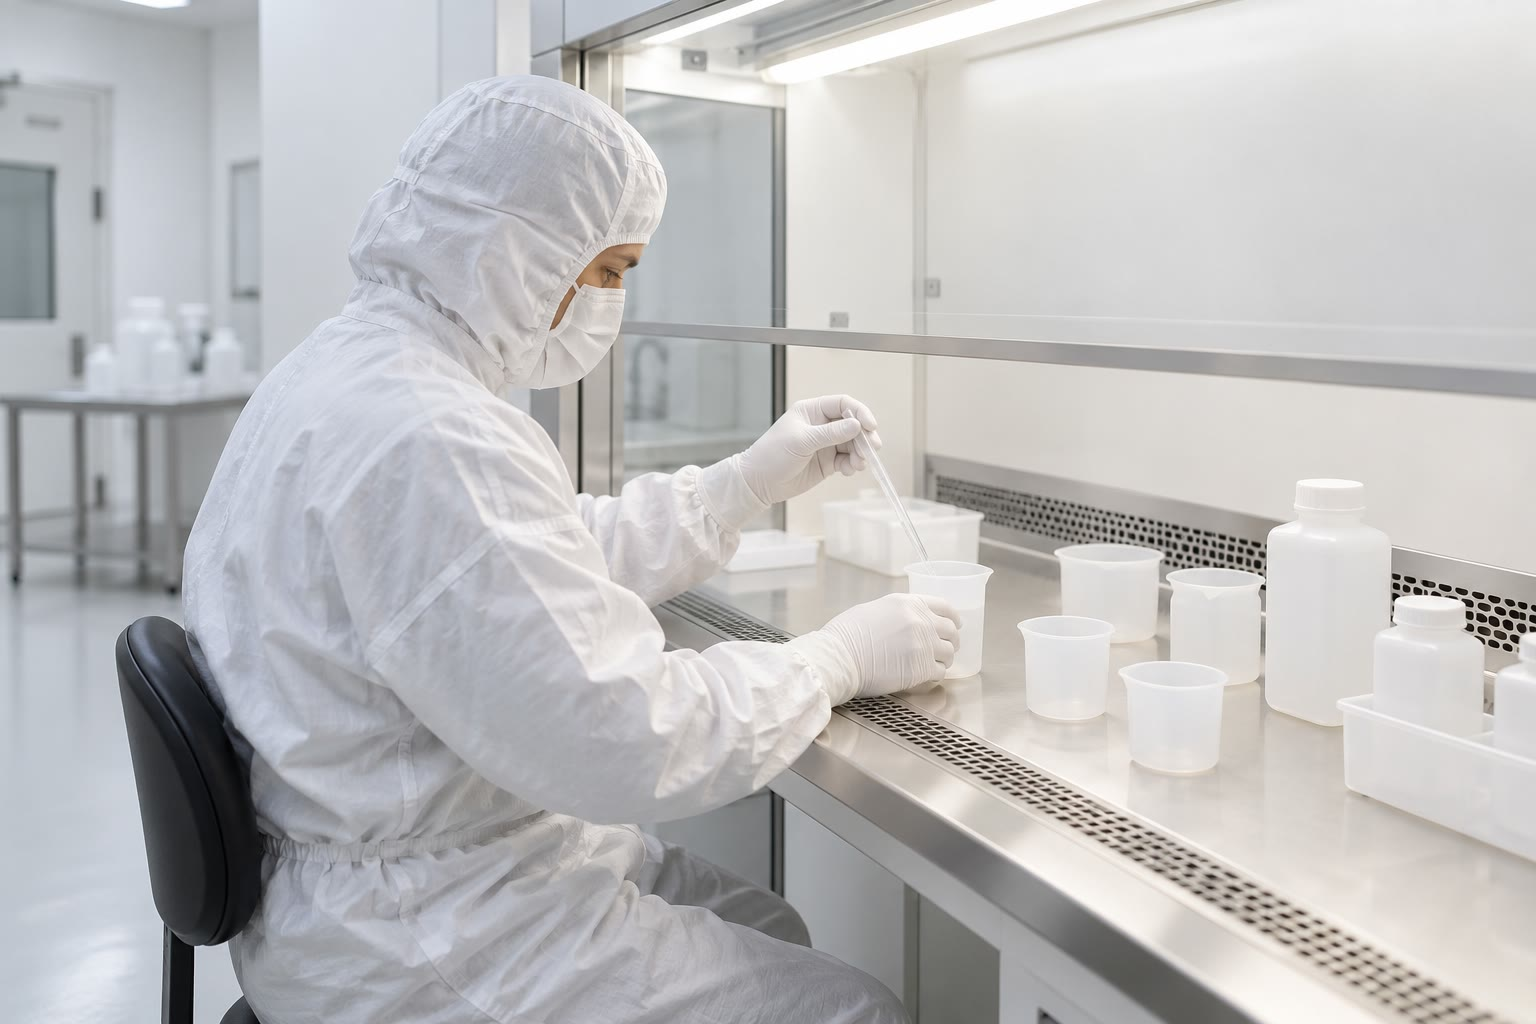
\includegraphics[width=\linewidth]{images/book4/ai/b2-clean-lab.jpg}

\smallskip
{\footnotesize Seorang pekerja berpakaian ruang bersih di meja aliran laminar sebuah
laboratorium bersih geokimia (ilustrasi buatan AI).\par}
\end{minipage}
\end{inthelab}
% ledger: usgs:bhvo2-trace, usgs:bhvo2-origin

\section{Latihan}

\begin{exercise}[$\star$]\label{exo:b2:elements-in-the-earth:1}
Basal BHVO-2 mengandung 0.5130 persen \ce{K2O} dan 2.731 persen \ce{TiO2}
menurut massa. Dengan massa atom K 39.10, Ti 47.87, dan O 16.00, hitunglah
kandungan kalium dan titaniumnya dalam ppm.
\end{exercise}

\begin{exercise}[$\star$]\label{exo:b2:elements-in-the-earth:2}
Dalam \omterm{def:b2:elements-in-the-earth:bse}{Bumi silikat total}, perbandingan $(X/\mathrm{Mg})$ dibagi perbandingan CI
bernilai 1.16 untuk aluminium, 0.22 untuk natrium, 0.077 untuk nikel, dan 0.0029 untuk
iridium. \omterm{def:b2:planet-formation-meteorites:condensation}{Suhu kondensasi} unsur-unsur ini adalah 1653, 958, 1353,
dan \qty{1603}{K}. Sebutkan kelas Goldschmidt setiap unsur dan jelaskan setiap
pengurasan.
\end{exercise}

\begin{exercise}[$\star$]\label{exo:b2:elements-in-the-earth:3}
Kerak benua atas mengandung \qty{31}{ppm} lantanum dan \qty{2.0}{ppm}
iterbium; \omterm{def:b2:elements-in-the-earth:ci}{kondrit CI} 0.232 dan \qty{0.163}{ppm}. Hitunglah nilai yang
dinormalisasi terhadap \omterm{def:b2:planet-formation-meteorites:chondrule}{kondrit} dan $(\mathrm{La}/\mathrm{Yb})_N$. Apa yang dikatakan
perbandingan itu tentang kerak?
\end{exercise}

\begin{exercise}[$\star$]\label{exo:b2:elements-in-the-earth:4}
Kerak benua atas mengandung 4.7, 1.0, dan \qty{4.0}{ppm} samarium,
europium, dan gadolinium; \omterm{def:b2:elements-in-the-earth:ci}{kondrit CI} 0.145, 0.0546, dan \qty{0.198}{ppm}.
Hitunglah $\mathrm{Eu}/\mathrm{Eu}^*$. Mineral apa yang menjelaskan hasilnya?
\end{exercise}

\begin{exercise}[$\star\star$]\label{exo:b2:elements-in-the-earth:5}
Sebuah piroksenit garnet terdiri atas 65 persen klinopiroksen, 18 persen garnet, dan
17 persen olivin, ortopiroksen, dan spinel. Koefisien partisi
lantanum adalah 0.058, 0.001, dan 0.001, koefisien partisi lutesium 0.53, 5.8, dan 0.18.
Hitunglah koefisien totalnya. Unsur mana yang kompatibel dalam batuan itu? Mineral
mana yang memuat sebagian besar lutesium batuan itu?
\end{exercise}

\begin{exercise}[$\star\star$]\label{exo:b2:elements-in-the-earth:6}
\omterm{def:b2:elements-in-the-earth:bse}{Bumi silikat total} mengandung 22.8 persen magnesium, \qty{2670}{ppm}
natrium, dan \qty{1960}{ppm} nikel; \omterm{def:b2:elements-in-the-earth:ci}{kondrit CI} 9.587 persen,
\qty{5010}{ppm}, dan \qty{10640}{ppm}. Hitunglah perbandingan ternormalisasi-Mg terhadap CI untuk
natrium dan nikel. Kedua unsur mengembun di sekitar \qty{1000}{K} atau lebih; mengapa
nikel lebih terkuras?
\end{exercise}

\begin{exercise}[$\star\star$]\label{exo:b2:elements-in-the-earth:7}
Sebuah klinopiroksen mengkristal dari lelehan berkomposisi MORB rata-rata,
\qty{5.21}{ppm} lantanum dan \qty{0.53}{ppm} lutesium. Koefisien
partisinya 0.058 untuk lantanum dan 0.53 untuk lutesium. Hitunglah kandungan
lantanum dan lutesiumnya, serta perbandingan $(\mathrm{La}/\mathrm{Lu})_N$
dalam kristal terhadap yang dalam lelehan (CI: La 0.232, Lu \qty{0.0237}{ppm}).
\end{exercise}

\begin{exercise}[$\star\star$]\label{exo:b2:elements-in-the-earth:8}
Dengan normalisasi terhadap \omterm{def:b2:elements-in-the-earth:bse}{mantel primitif} (Nb \qty{0.658}{ppm}, La \qty{0.648}{ppm}),
hitunglah $(\mathrm{Nb}/\mathrm{La})_N$ untuk kerak benua atas (Nb 12,
La \qty{31}{ppm}), basal Hawaii (18.10, \qty{15.20}{ppm}), dan MORB rata-rata
(5.24, \qty{5.21}{ppm}). Mana di antaranya yang membawa ciri zona subduksi?
\end{exercise}

\begin{exercise}[$\star\star$]\label{exo:b2:elements-in-the-earth:9}
Kalium dan uranium sama-sama sangat inkompatibel. Hitunglah perbandingan massa K/U dalam
\omterm{def:b2:elements-in-the-earth:bse}{mantel primitif} (K \qty{240}{ppm}, U \qty{0.0203}{ppm}), dalam MORB rata-rata
(\qty{0.160}{\percent} \ce{K2O}, U \qty{0.119}{ppm}), dan dalam kerak benua
atas (\qty{2.80}{\percent} \ce{K2O}, U \qty{2.7}{ppm}), dengan
$\mathrm{K}/\ce{K2O} = 0.830$ menurut massa. Apa arti perbandingan yang nyaris tetap itu,
dan mengapa K/U berguna untuk menaksir kalium sebuah planet?
\end{exercise}

\begin{exercise}[$\star\star\star$]\label{exo:b2:elements-in-the-earth:10}
Sejumlah kecil lelehan berada dalam kesetimbangan dengan piroksenit garnet pada latihan
5. Tunjukkan bahwa, untuk dua unsur, perbandingan
$(C_1/C_2)_{\mathrm{melt}}/(C_1/C_2)_{\mathrm{rock}}$ sama dengan
$\bar D_2/\bar D_1$. Hitunglah nilainya untuk lantanum dan lutesium, dan jelaskan mengapa
lelehan dari mantel yang mengandung garnet memiliki pola tanah jarang yang curam.
\end{exercise}

\begin{exercise}[$\star\star\star$]\label{exo:b2:elements-in-the-earth:11}
MORB rata-rata (Th \qty{0.404}{ppm}, Nb \qty{5.24}{ppm}) mengasimilasi kerak benua
atas (Th \qty{10.5}{ppm}, Nb \qty{12}{ppm}): fraksi massa $f$
kerak bercampur dengan $1-f$ basal. Tunjukkan bahwa konsentrasi campuran itu
linear terhadap $f$, tetapi perbandingan Th/Nb-nya tidak. Tentukan $f$ yang membuat Th/Nb mencapai
0.2, dan perbandingannya untuk $f = 0.1$.
\end{exercise}

\begin{exercise}[$\star\star\star$]\label{exo:b2:elements-in-the-earth:12}
Membuang air, karbon, atau inti logam yang tidak mengandung aluminium maupun
magnesium tidak mengubah perbandingan Al/Mg sisanya: tunjukkan hal itu. Dalam \omterm{def:b2:elements-in-the-earth:bse}{Bumi
silikat total}, $(\mathrm{Al}/\mathrm{Mg})$ bernilai 1.16 kali nilai CI. Jika
Bumi mempertahankan seluruh aluminiumnya, berapa bagian magnesium kondritiknya yang
hilang dari Bumi silikat? Dengan perbandingan ternormalisasi-Mg silikon,
0.83, berapa bagian silikon kondritiknya yang akan hilang dengan
anggapan yang sama?
\end{exercise}

\section{Soal: Menimbang inti dengan sebuah kondrit}

\begin{problem}[{Soal akhir pekan --- merekonstruksi Bumi total dari kondrit CI,
mantel, dan inti, serta menimbang inti}]
\label{pb:b2:elements-in-the-earth:1}
Seorang ahli geokimia planet ingin menimbang inti Bumi tanpa seismologi, hanya dari
kimia. Ia mengambil \omterm{def:b2:elements-in-the-earth:ci}{kondrit CI} sebagai bahan awal
(Mg \qty{95870}{ppm}, Al 8500, Si \num{106500}, Fe \num{182800},
Ni \qty{10640}{ppm}), \omterm{def:b2:elements-in-the-earth:bse}{mantel primitif} untuk Bumi silikat (MgO 37.8, FeO
8.05, NiO 0.25 persen; Mg 22.8, Si 21.0 persen), dan model inti yang terdiri atas 85.5
persen Fe, 5.2 persen Ni, dan 6.0 persen Si. Massa atom: Mg 24.31,
Si 28.09, Fe 55.85, Ni 58.69, O 16.00. Massa Bumi
\qty{5.972e24}{kg}.

\medskip\noindent\textbf{Bagian I --- Titik awal kondritik.}
\begin{enumerate}
\item Hitunglah perbandingan massa Fe/Mg, Ni/Mg, Si/Mg, dan Al/Mg \omterm{def:b2:elements-in-the-earth:ci}{kondrit CI}.
\item Ubahlah Fe/Si menjadi perbandingan atom. Spektroskopi fotosfer Matahari
memberikan 0.81 atom besi per atom silikon: apakah perbandingan itu masuk akal?
\item \omterm{def:b2:elements-in-the-earth:ci}{Kondrit CI} mengandung 2.1 persen hidrogen dan 3.5 persen karbon, yang terikat dalam
mineral yang mengandung air dan senyawa organik yang tidak dipertahankan Bumi. Mengapa
perbandingan pada pertanyaan 1 tidak perlu dikoreksi untuk kehilangan ini?
\item Mengapa magnesium merupakan unsur acuan yang cocok untuk soal inti, dan
mengapa besi tidak dapat dipakai?
\item Nikel, magnesium, besi, dan silikon mengembun dalam rentang \qty{50}{K} satu sama
lain (1353, 1336, 1334, dan \qty{1310}{K}). Mengapa hal ini mendukung
anggapan bahwa Bumi total mempertahankan perbandingan kondritiknya? Perbandingan mana pada
pertanyaan 1 yang menyimpang dari kelompok ini, dan apa kata bab ini tentangnya?
\end{enumerate}

\noindent\textbf{Bagian II --- Bumi silikat.}
\begin{enumerate}[resume]
\item Ubahlah FeO dan NiO \omterm{def:b2:elements-in-the-earth:bse}{mantel primitif} menjadi Fe dan Ni.
\item Hitunglah Fe/Mg dan Ni/Mg dalam Bumi silikat.
\item Berapa bagian Fe dan Ni kondritik yang hilang dari Bumi
silikat, pada magnesium tetap?
\item Perhitungan yang sama untuk iridium (\omterm{def:b2:elements-in-the-earth:bse}{mantel primitif} \qty{3.2}{ppb}, CI
\qty{0.470}{ppm}) memberikan bagian yang hilang sebesar 99.7 persen. Mengapa bagian itu lebih besar
daripada untuk nikel, dan bagian nikel lebih besar daripada untuk besi?
\item Di mana besi berada dalam Bumi silikat, dan mengapa tidak seluruhnya masuk ke
inti?
\end{enumerate}

\noindent\textbf{Bagian III --- Menimbang inti.}
\begin{enumerate}[resume]
\item Tuliskan neraca besi Bumi dengan fraksi massa inti $x$, dan
turunkan \cref{prop:b2:elements-in-the-earth:core}.
\item Hitunglah $y = x/(1-x)$ dan $x$ dari besi.
\item Lakukan hal yang sama dari nikel.
\item Kedua taksiran itu tidak tepat sama. Gabungkan keduanya dengan kuadrat terkecil:
minimumkan $\sum (a_iy - b_i)^2$, dengan $a_i y = b_i$ adalah dua persamaan pada
pertanyaan 12 dan 13, lalu berikan $y$ dan $x$ terbaik.
\item Mengapa nilai kuadrat terkecil itu begitu dekat dengan taksiran dari besi?
\item Dari kedua persamaan itu, hitunglah perbandingan Fe/Ni inti yang akan membuat
keduanya tepat. Bandingkan dengan model inti.
\item Berikan massa inti.
\end{enumerate}

\noindent\textbf{Bagian IV --- Pemeriksaan dan konsekuensi.}
\begin{enumerate}[resume]
\item Seismologi memberikan inti sebesar 32.5 persen massa Bumi. Berapa
persen selisih taksiran kimia dari nilai itu?
\item Dengan inti sebesar 32.5 persen, berapa banyak besi yang harus dikandung inti untuk
menutup neraca besi? Apakah hal ini sesuai dengan inti yang 10 persennya unsur
ringan?
\item Model inti mengandung 9.3 persen unsur selain Fe dan Ni. Unsur ringan mana
yang menjadi calon, dan bukti apa dalam bab ini yang mendukung silikon?
\item Dengan $y$ dari pertanyaan 14, hitunglah kandungan silikon inti yang akan
membuat Si/Mg Bumi total kondritik.
\item Bandingkan dengan 6 persen pada model. Kemukakan suatu alasan, dari bab
sebelumnya, mengapa sebagian silikon mungkin hilang dari Bumi sama sekali.
\item Model inti mengandung \qty{0.5}{ppm} emas, \omterm{def:b2:elements-in-the-earth:bse}{mantel primitif}
\qty{1}{ppb}. Dengan inti sebesar 32.5 persen, berapa bagian emas Bumi yang
berada di inti?
\item Nyatakan fraksi massa inti Bumi yang diperoleh dari kimia saja,
angka kunci soal ini.
\end{enumerate}
\end{problem}
% ledger: lodders:ci-table, lodders:ci-h-photo, ms95:pm-oxides, ms95:pm-trace, mcd03:core, earth:mass, badro:core, lodders:tc-table
